\section{Example}
\label{example}

In this section, we present an example app to motivate our technique for automatically testing %to illustrate how we leverage specific
user-interaction features of mobile apps. % to automatically find bugs.
For illustration, %this example, 
we use a real bug from Kitchen Timer, an open source Android app. As the name suggests, Kitchen Timer is a timer for cooking. It contains three timers which can be set independently and go off by sounding an alarm after counting down to zero. In addition, Kitchen Timer provides other functionalities to change Preferences (e.g., the alarm sound, the LED color, timer names), save preset timers, and many more. 

While we used the complete Kitchen Timer for the bug study and evaluation (Sections~\ref{study} and \ref{evaluation}), we describe a simplified version for the sake of this example. Figure~\ref{fig:kitchenTimer} shows snapshots of Kitchen Timer. In this simplified Kitchen Timer, the user can set one timer by using the plus and minus signs on the main screen (Figure~\ref{fig:mainTimers}). The numbers from left to right show the hours, minutes, and seconds for the timer to be set. Then the user can start the timer by hitting the Start button (to get to Figure~\ref{fig:timerRunning}) or stop it by hitting the Stop button. Furthermore, he can select Info, Preferences, or Donation from the menu (to get to Figures~\ref{fig:info}, \ref{fig:prefs} and \ref{fig:donation}). All of these screens support rotation. For simplicity, we excluded further actions from Info, Preferences, and Donation from the simplified app. The user can, however, go back to the main screen from them.

\begin{figure}[!t]
\centering
\subfloat[\scriptsize Main Timers]{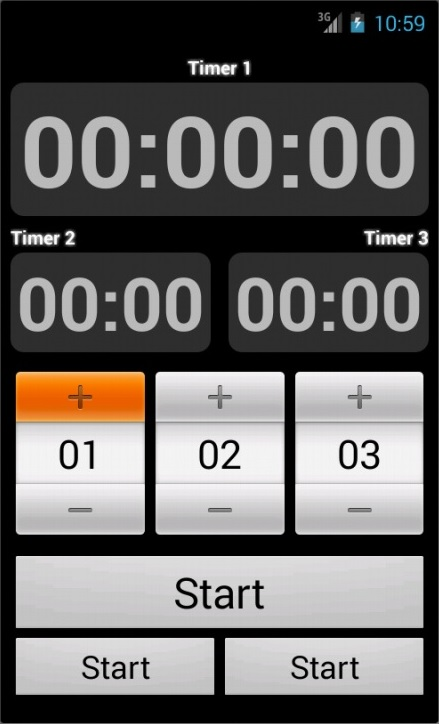
\includegraphics[width=0.18\columnwidth]{figures/before.jpg}
\label{fig:mainTimers}
}
\hfill
\subfloat[Timer Running]{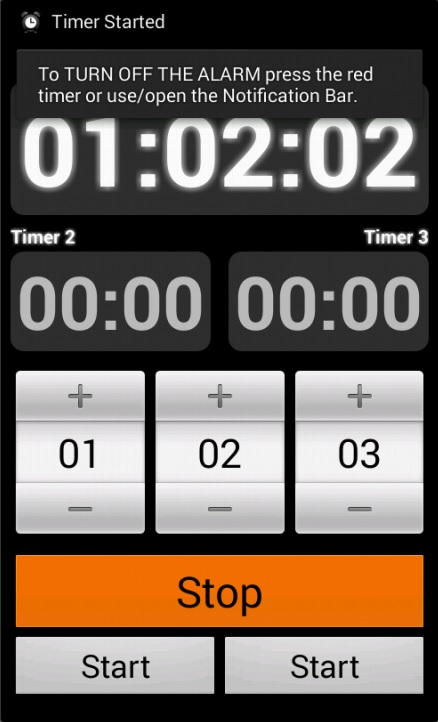
\includegraphics[width=0.18\columnwidth]{figures/timerRunning.jpg}
\label{fig:timerRunning}
}
\hfill
\subfloat[Info]{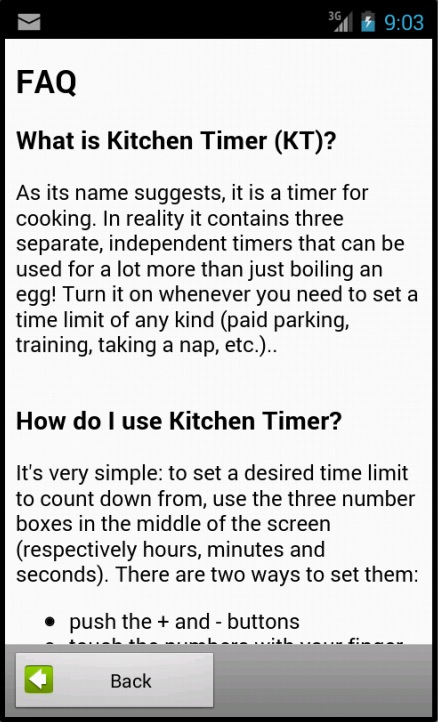
\includegraphics[width=0.18\columnwidth]{figures/info.jpg}
\label{fig:info}
}
\hfill
\subfloat[Preferences]{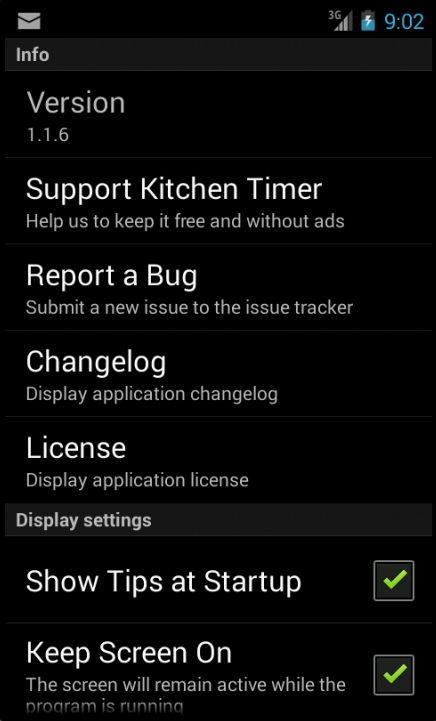
\includegraphics[width=0.18\columnwidth]{figures/prefs.jpg}
\label{fig:prefs}
}
\hfill
\subfloat[Donation]{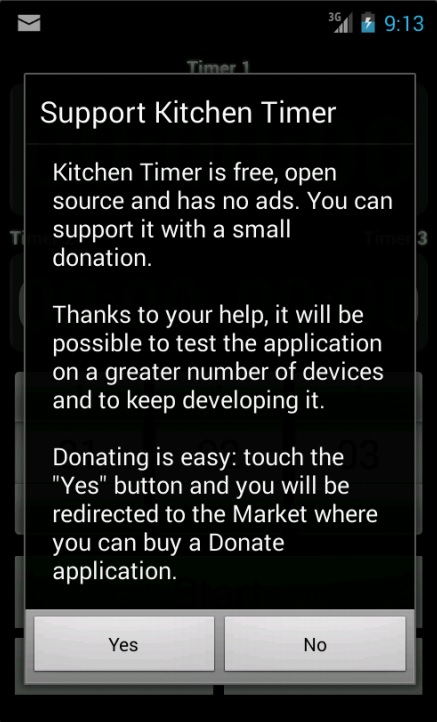
\includegraphics[width=0.18\columnwidth]{figures/donation.jpg}
\label{fig:donation}
}
\caption{Snapshots of Simplified Kitchen Timer.}
\label{fig:kitchenTimer}
\end{figure}

\begin{figure}[!t]
\centering
\subfloat[The user sets a timer.]{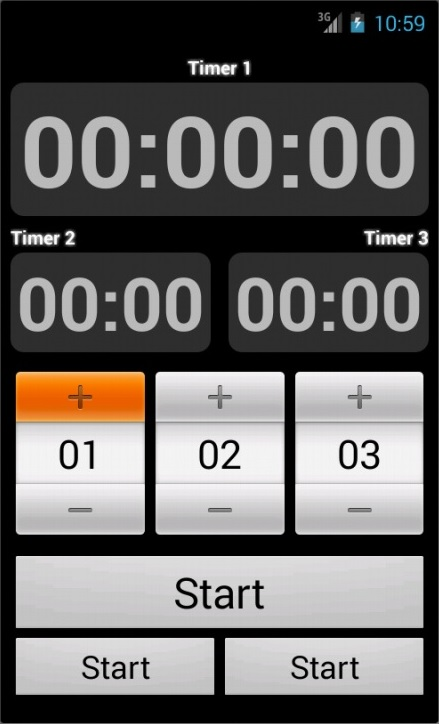
\includegraphics[width=0.3\columnwidth]{figures/before.jpg}
\label{fig:example_c}
}
\hfil
\subfloat[Values overwritten after two rotations.]{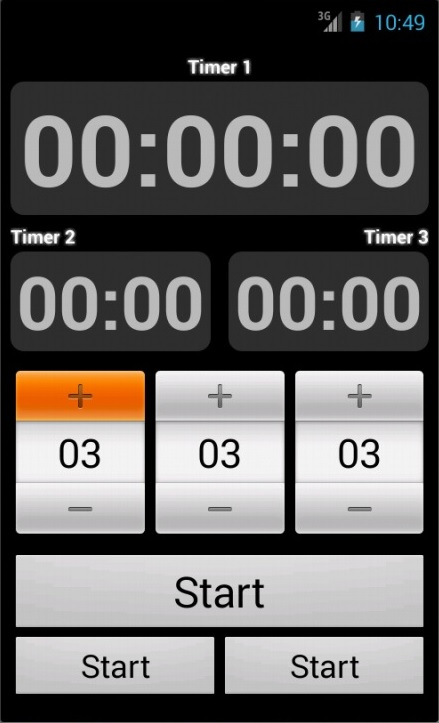
\includegraphics[width=0.3\columnwidth]{figures/after.jpg}
\label{fig:example_d}
}
\caption{Snapshots of a Bug in Kitchen Timer.}
\label{fig:example}
\end{figure}


As Figure~\ref{fig:example} depicts, Kitchen Timer has a bug that is manifested when the device is rotated twice. If the user sets a timer (Figure~\ref{fig:example_c}), and then rotates the mobile device twice before starting the timer (Figure~\ref{fig:example_d}), the value of seconds overwrites the values of minutes and hours, here changing the timer from 1 hour, 2 minutes, and 3 seconds to 3 hours, 3 minutes, and 3 seconds.

%OLD: belongs to the example app I wrote not kitchen timer
%This bug, similar to most of the rotation bugs we saw in the bug study, is an error of omission, i.e., the programmer neglects that the \texttt{onCreate} method is called after rotation and does not retrieve the data entered into the text box in this method. Hence, traditional adequacy criteria such as 100\% line coverage cannot catch this bug since they focus on errors of commission, i.e., when the programmer does something but incorrectly. GUI based event sequences can, in principle, find such bugs. Yet as apps grow more complicated, event sequences of bigger sizes are required to find bugs, resulting in state space explosion. In addition, automatic test sequence generation techniques which aim these adequacy criteria do not provide automatic oracles, only test sequences. 
Our tool automatically finds this bug. % by particularly noting the fact that, unlike traditional computers, a mobile device can be rotated and is expected to behave properly. 

%OLD: belongs to the example app I wrote not kitchen timer
%This app has an activity life-cycle bug too. The app should show a welcome message the very first time it is run (Figure~\ref{fig:eample_a}). Upon the first launch, the app saves its status in a file to avoid showing the welcome message again (as is commonly done in Android apps). However, the app wrongly uses two different file names for reading and writing. If the app is killed, garbage collected, and restarted, the bug is revealed by showing the welcome message even though it is not the first run, since the app fails to read the status from the file. This is indeed a subtle activity life-cycle bug: It is possible to kill the app (through the \texttt{onDestroy} method) and then restart it before the app gets garbage collected, without manifesting the bug. (The reason is that static variables including the one that keeps the status still have the values they had before killing the app.) Our tool shows this bug by thorough testing of the activity life-cycle. Event sequences, which usually do not include system level events such as killing apps, cannot find this bug. While 100\% line coverage shows this bug, in practice it is rare that full line coverage is achieved. Furthermore, automatic test sequence generation methods that aim such criteria do not provide an automatic oracle and the user has to manually write the oracle/check the results.
